\documentclass{standalone}
\usepackage{tikz}
\usetikzlibrary{patterns, positioning}

\begin{document}
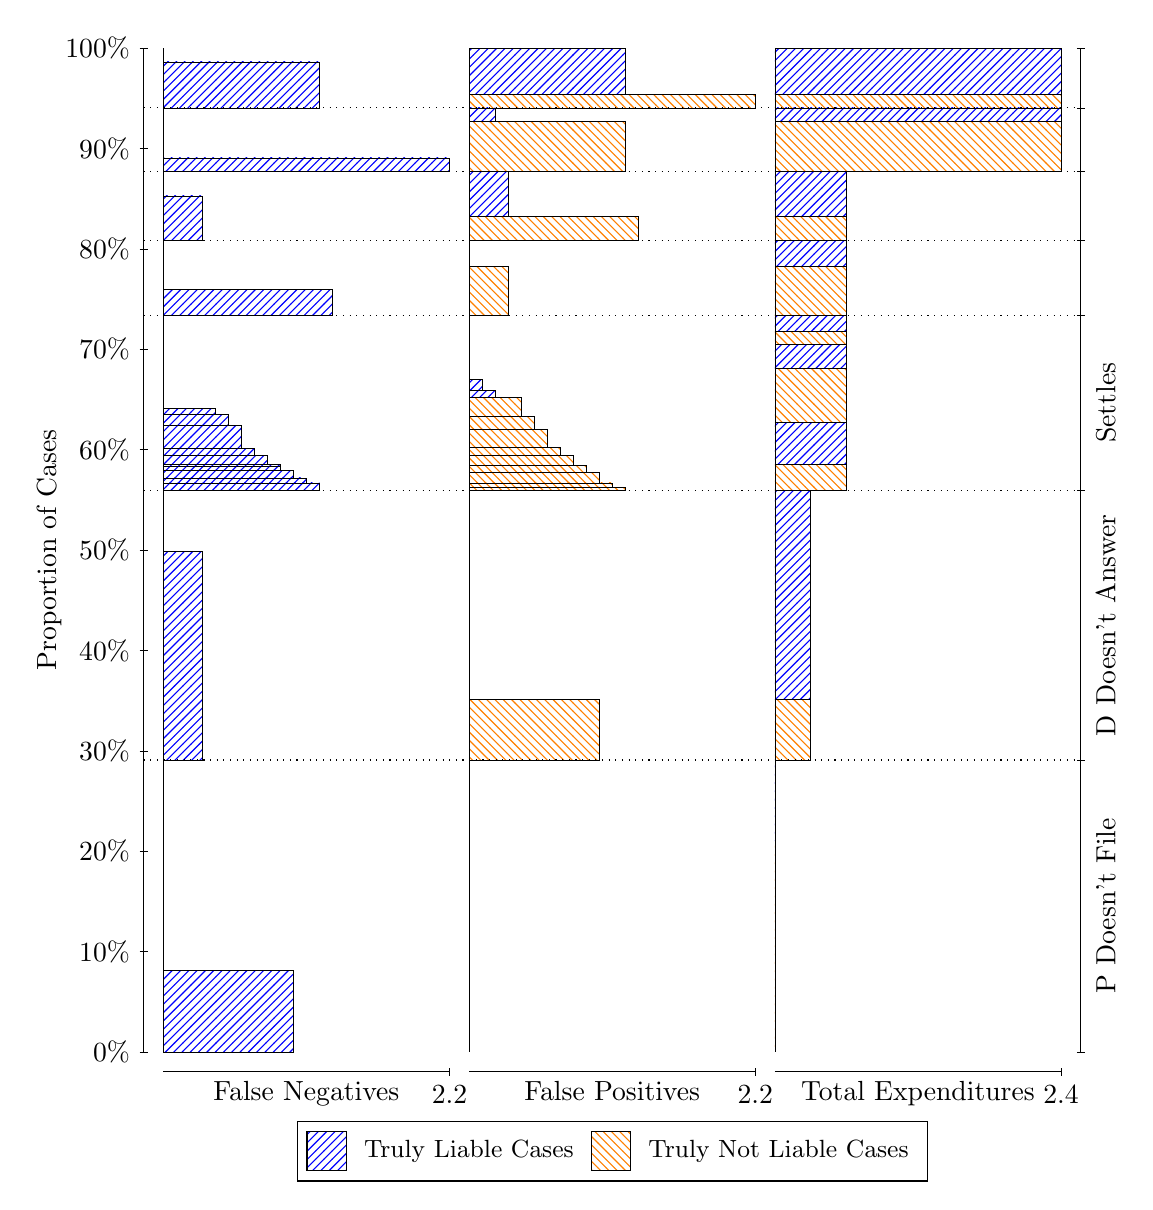
\begin{tikzpicture}
\draw[black, very thin] (1.5,1.75) -- (1.5,14.5);
\node[rotate=90, anchor=center] at (0.3, 8.125) {Proportion of Cases};
\draw[black, very thin] (1.45,1.75) -- (1.55,1.75);
\node[anchor=east] at (1.45, 1.75) {0\%};
\draw[black, very thin] (1.45,3.025) -- (1.55,3.025);
\node[anchor=east] at (1.45, 3.025) {10\%};
\draw[black, very thin] (1.45,4.3) -- (1.55,4.3);
\node[anchor=east] at (1.45, 4.3) {20\%};
\draw[black, very thin] (1.45,5.575) -- (1.55,5.575);
\node[anchor=east] at (1.45, 5.575) {30\%};
\draw[black, very thin] (1.45,6.85) -- (1.55,6.85);
\node[anchor=east] at (1.45, 6.85) {40\%};
\draw[black, very thin] (1.45,8.125) -- (1.55,8.125);
\node[anchor=east] at (1.45, 8.125) {50\%};
\draw[black, very thin] (1.45,9.4) -- (1.55,9.4);
\node[anchor=east] at (1.45, 9.4) {60\%};
\draw[black, very thin] (1.45,10.675) -- (1.55,10.675);
\node[anchor=east] at (1.45, 10.675) {70\%};
\draw[black, very thin] (1.45,11.95) -- (1.55,11.95);
\node[anchor=east] at (1.45, 11.95) {80\%};
\draw[black, very thin] (1.45,13.225) -- (1.55,13.225);
\node[anchor=east] at (1.45, 13.225) {90\%};
\draw[black, very thin] (1.45,14.5) -- (1.55,14.5);
\node[anchor=east] at (1.45, 14.5) {100\%};

\draw[black, very thin] (13.4,1.75) -- (13.4,14.5);
\draw[black, very thin] (13.35,1.75) -- (13.45,1.75);
\node[anchor=west] at (13.35, 1.75) {};
\draw[black, very thin] (13.35,5.4584) -- (13.45,5.4584);
\node[anchor=west] at (13.35, 5.4584) {};
\draw[black, very thin] (13.35,8.8834) -- (13.45,8.8834);
\node[anchor=west] at (13.35, 8.8834) {};
\draw[black, very thin] (13.35,11.107) -- (13.45,11.107);
\node[anchor=west] at (13.35, 11.107) {};
\draw[black, very thin] (13.35,12.055) -- (13.45,12.055);
\node[anchor=west] at (13.35, 12.055) {};
\draw[black, very thin] (13.35,12.929) -- (13.45,12.929);
\node[anchor=west] at (13.35, 12.929) {};
\draw[black, very thin] (13.35,13.741) -- (13.45,13.741);
\node[anchor=west] at (13.35, 13.741) {};
\draw[black, very thin] (13.35,14.5) -- (13.45,14.5);
\node[anchor=west] at (13.35, 14.5) {};

\draw[black, very thin, pattern color=blue, pattern=north east lines] (1.75,1.75) rectangle (3.4015,2.7814);
\draw[black, very thin, pattern color=orange, pattern=north west lines] (1.75,2.7814) rectangle (1.75,5.4584);
\draw[black, very thin, pattern color=blue, pattern=north east lines] (1.75,5.4584) rectangle (2.2455,8.1095);
\draw[black, very thin, pattern color=orange, pattern=north west lines] (1.75,8.1095) rectangle (1.75,8.8834);
\draw[black, very thin, pattern color=blue, pattern=north east lines] (1.75,8.8834) rectangle (3.7318,8.9762);
\draw[black, very thin, pattern color=blue, pattern=north east lines] (1.75,8.9762) rectangle (3.5667,9.0417);
\draw[black, very thin, pattern color=blue, pattern=north east lines] (1.75,9.0417) rectangle (3.4015,9.1339);
\draw[black, very thin, pattern color=blue, pattern=north east lines] (1.75,9.1339) rectangle (3.2364,9.1821);
\draw[black, very thin, pattern color=blue, pattern=north east lines] (1.75,9.1821) rectangle (3.2364,9.2111);
\draw[black, very thin, pattern color=blue, pattern=north east lines] (1.75,9.2111) rectangle (3.0712,9.3252);
\draw[black, very thin, pattern color=blue, pattern=north east lines] (1.75,9.3252) rectangle (2.9061,9.4151);
\draw[black, very thin, pattern color=blue, pattern=north east lines] (1.75,9.4151) rectangle (2.7409,9.7037);
\draw[black, very thin, pattern color=blue, pattern=north east lines] (1.75,9.7037) rectangle (2.5758,9.8424);
\draw[black, very thin, pattern color=blue, pattern=north east lines] (1.75,9.8424) rectangle (2.4106,9.9259);
\draw[black, very thin, pattern color=orange, pattern=north west lines] (1.75,9.9259) rectangle (1.75,11.107);
\draw[black, very thin, pattern color=blue, pattern=north east lines] (1.75,11.107) rectangle (3.897,11.432);
\draw[black, very thin, pattern color=orange, pattern=north west lines] (1.75,11.432) rectangle (1.75,12.055);
\draw[black, very thin, pattern color=blue, pattern=north east lines] (1.75,12.055) rectangle (2.2455,12.622);
\draw[black, very thin, pattern color=orange, pattern=north west lines] (1.75,12.622) rectangle (1.75,12.929);
\draw[black, very thin, pattern color=blue, pattern=north east lines] (1.75,12.929) rectangle (5.3833,13.105);
\draw[black, very thin, pattern color=orange, pattern=north west lines] (1.75,13.105) rectangle (1.75,13.741);
\draw[black, very thin, pattern color=blue, pattern=north east lines] (1.75,13.741) rectangle (3.7318,14.325);
\draw[black, very thin, pattern color=orange, pattern=north west lines] (1.75,14.325) rectangle (1.75,14.5);
\draw[black, very thin, pattern color=orange, pattern=north west lines] (5.6333,1.75) rectangle (5.6333,4.427);
\draw[black, very thin, pattern color=blue, pattern=north east lines] (5.6333,4.427) rectangle (5.6333,5.4584);
\draw[black, very thin, pattern color=orange, pattern=north west lines] (5.6333,5.4584) rectangle (7.2848,6.2324);
\draw[black, very thin, pattern color=blue, pattern=north east lines] (5.6333,6.2324) rectangle (5.6333,8.8834);
\draw[black, very thin, pattern color=orange, pattern=north west lines] (5.6333,8.8834) rectangle (7.6152,8.9167);
\draw[black, very thin, pattern color=orange, pattern=north west lines] (5.6333,8.9167) rectangle (7.45,8.9783);
\draw[black, very thin, pattern color=orange, pattern=north west lines] (5.6333,8.9783) rectangle (7.2848,9.1078);
\draw[black, very thin, pattern color=orange, pattern=north west lines] (5.6333,9.1078) rectangle (7.1197,9.1963);
\draw[black, very thin, pattern color=orange, pattern=north west lines] (5.6333,9.1963) rectangle (6.9545,9.3308);
\draw[black, very thin, pattern color=orange, pattern=north west lines] (5.6333,9.3308) rectangle (6.7894,9.433);
\draw[black, very thin, pattern color=orange, pattern=north west lines] (5.6333,9.433) rectangle (6.6242,9.6616);
\draw[black, very thin, pattern color=orange, pattern=north west lines] (5.6333,9.6616) rectangle (6.4591,9.8204);
\draw[black, very thin, pattern color=orange, pattern=north west lines] (5.6333,9.8204) rectangle (6.2939,10.065);
\draw[black, very thin, pattern color=blue, pattern=north east lines] (5.6333,10.065) rectangle (5.9636,10.149);
\draw[black, very thin, pattern color=blue, pattern=north east lines] (5.6333,10.149) rectangle (5.7985,10.287);
\draw[black, very thin, pattern color=blue, pattern=north east lines] (5.6333,10.287) rectangle (5.6333,11.107);
\draw[black, very thin, pattern color=orange, pattern=north west lines] (5.6333,11.107) rectangle (6.1288,11.731);
\draw[black, very thin, pattern color=blue, pattern=north east lines] (5.6333,11.731) rectangle (5.6333,12.055);
\draw[black, very thin, pattern color=orange, pattern=north west lines] (5.6333,12.055) rectangle (7.7803,12.363);
\draw[black, very thin, pattern color=blue, pattern=north east lines] (5.6333,12.363) rectangle (6.1288,12.929);
\draw[black, very thin, pattern color=orange, pattern=north west lines] (5.6333,12.929) rectangle (7.6152,13.565);
\draw[black, very thin, pattern color=blue, pattern=north east lines] (5.6333,13.565) rectangle (5.9636,13.741);
\draw[black, very thin, pattern color=orange, pattern=north west lines] (5.6333,13.741) rectangle (9.2667,13.916);
\draw[black, very thin, pattern color=blue, pattern=north east lines] (5.6333,13.916) rectangle (7.6152,14.5);
\draw[black, very thin, pattern color=orange, pattern=north west lines] (9.5167,1.75) rectangle (9.5167,4.427);
\draw[black, very thin, pattern color=blue, pattern=north east lines] (9.5167,4.427) rectangle (9.5167,5.4584);
\draw[black, very thin, pattern color=orange, pattern=north west lines] (9.5167,5.4584) rectangle (9.9708,6.2324);
\draw[black, very thin, pattern color=blue, pattern=north east lines] (9.5167,6.2324) rectangle (9.9708,8.8834);
\draw[black, very thin, pattern color=orange, pattern=north west lines] (9.5167,8.8834) rectangle (10.425,9.2091);
\draw[black, very thin, pattern color=blue, pattern=north east lines] (9.5167,9.2091) rectangle (10.425,9.7505);
\draw[black, very thin, pattern color=orange, pattern=north west lines] (9.5167,9.7505) rectangle (10.425,10.435);
\draw[black, very thin, pattern color=blue, pattern=north east lines] (9.5167,10.435) rectangle (10.425,10.734);
\draw[black, very thin, pattern color=orange, pattern=north west lines] (9.5167,10.734) rectangle (10.425,10.905);
\draw[black, very thin, pattern color=blue, pattern=north east lines] (9.5167,10.905) rectangle (10.425,11.107);
\draw[black, very thin, pattern color=orange, pattern=north west lines] (9.5167,11.107) rectangle (10.425,11.731);
\draw[black, very thin, pattern color=blue, pattern=north east lines] (9.5167,11.731) rectangle (10.425,12.055);
\draw[black, very thin, pattern color=orange, pattern=north west lines] (9.5167,12.055) rectangle (10.425,12.363);
\draw[black, very thin, pattern color=blue, pattern=north east lines] (9.5167,12.363) rectangle (10.425,12.929);
\draw[black, very thin, pattern color=orange, pattern=north west lines] (9.5167,12.929) rectangle (13.15,13.565);
\draw[black, very thin, pattern color=blue, pattern=north east lines] (9.5167,13.565) rectangle (13.15,13.741);
\draw[black, very thin, pattern color=orange, pattern=north west lines] (9.5167,13.741) rectangle (13.15,13.916);
\draw[black, very thin, pattern color=blue, pattern=north east lines] (9.5167,13.916) rectangle (13.15,14.5);
\draw[black, dotted] (1.5,5.4584) -- (13.4,5.4584);
\draw[black, dotted] (1.5,8.8834) -- (13.4,8.8834);
\draw[black, dotted] (1.5,11.107) -- (13.4,11.107);
\draw[black, dotted] (1.5,12.055) -- (13.4,12.055);
\draw[black, dotted] (1.5,12.929) -- (13.4,12.929);
\draw[black, dotted] (1.5,13.741) -- (13.4,13.741);
\draw[black, very thin] (1.75,1.5) -- (5.3833,1.5);
\node[anchor=north] at (3.5667, 1.5) {False Negatives};
\draw[black, very thin] (5.3833,1.45) -- (5.3833,1.55);
\node[anchor=north] at (5.3833, 1.45) {2.2};

\draw[black, very thin] (5.6333,1.5) -- (9.2667,1.5);
\node[anchor=north] at (7.45, 1.5) {False Positives};
\draw[black, very thin] (9.2667,1.45) -- (9.2667,1.55);
\node[anchor=north] at (9.2667, 1.45) {2.2};

\draw[black, very thin] (9.5167,1.5) -- (13.15,1.5);
\node[anchor=north] at (11.333, 1.5) {Total Expenditures};
\draw[black, very thin] (13.15,1.45) -- (13.15,1.55);
\node[anchor=north] at (13.15, 1.45) {2.4};

\node[black, centered, rotate=90] at (13.72, 3.6042) {P Doesn't File};
\node[black, centered, rotate=90] at (13.72, 7.1709) {D Doesn't Answer};
\node[black, centered, rotate=90] at (13.72, 9.9954) {Settles};





\draw (7.449999999999999,1.5) node[draw=none] (baseCoordinate) {};
\begin{scope}[align=center]
        \matrix[scale=0.5, draw=black, below=0.5cm of baseCoordinate, nodes={draw}, column sep=0.1cm]{
            \node[rectangle, draw, minimum width=0.5cm, minimum height=0.5cm, pattern=north east lines, pattern color=blue] {}; &
            \node[draw=none, font=\small] (B) {Truly Liable Cases}; &
            \node[rectangle, draw, minimum width=0.5cm, minimum height=0.5cm, pattern=north west lines, pattern color=orange] {}; &
            \node[draw=none, font=\small] (B) {Truly Not Liable Cases}; \\
            };
\end{scope}

\end{tikzpicture}
\end{document}